\setstretch{1.2}%řádkování
\hspace{1 cm}
Pro vývoj mobilní aplikace byl zvolen \textbf{React Native}, protože se jedná o moderní a multiplatformní nástroj pro tvorbu mobilních aplikací. Jako programovací jazyk pro tvorbu aplikace byl zvolen \textbf{TypeScript} a jako jazyk pro tvorbu kódu pro \textbf{Arduino} byl zvolen \textbf{Wiring}.

\begin{itemize}
    \item \textbf{Mobilní aplikace:} Je strukturována do komponent, které jsou importovány do hlavního souboru \texttt{App.tsx}. Každá komponenta má svůj vlastní soubor (ve složce Moje\_Komponenty) a obsahuje kód pro určitou část uživatelského rozhraní nebo funkcionalitu aplikace. Hlavní komponenta \texttt{App.tsx} je zodpovědná za celkové uspořádání aplikace a její vzhled (například změna vzhledu v závislosti na tmavém či světlém režimu zařízení). Komponenta \texttt{ConnectToHC05} je zodpovědná za skenování dostupných Bluetooth zařízení a připojení k zařízení HC-05. Tato komponenta využívá knihovnu \texttt{react-native-ble-plx} pro komunikaci s Bluetooth zařízením. Po úspěšném připojení k zařízení HC-05 se aktualizují stavové proměnné \texttt{connected} a \texttt{deviceName}. Komponenty \texttt{TlacitkoBluetooth} a \texttt{TlacitkoSoubory} jsou tlačítka, která uživatel může stisknout pro připojení k Bluetooth zařízení a pro export souborů z SD karty. Komponenta \texttt{RequestPermissions.tsx} je zodpovědná za požadování oprávnění k užití polohy pro použití Bluetooth.
    
    \item \textbf{Arduino kód:} Je napsán v jazyce \textbf{Wiring}, který vychází z jazyka \textbf{C++}. Na začádku kódu jsou definovány vstupní a výstupní piny a jsou importovány potřebné knihovny. Dále je kód je strukturován do dvou hlavních funkcí: \texttt{setup()} a \texttt{loop()}. 

    Funkce \texttt{setup()} je volána jednou při startu programu. V této funkci se inicializuje komunikace s Bluetooth modulem a SD kartou. Dále se čtou názvy souborů na SD kartě a ukládají se do pole \texttt{filenames}.

    Funkce \texttt{loop()} je poté volána opakovaně. Tato funkce kontroluje, zda jsou k dispozici data z Bluetooth modulu. Pokud ano, načte první znak ve frontě a dekóduje ho na číslo, které odpovídá indexu souboru v poli \texttt{filenames}. Poté otevře tento soubor na SD kartě a vypíše jeho obsah přes Bluetooth. Pokud se nepodaří otevřít soubor, vypíše chybovou zprávu.

    \begin{figure}[H]
        \centering
        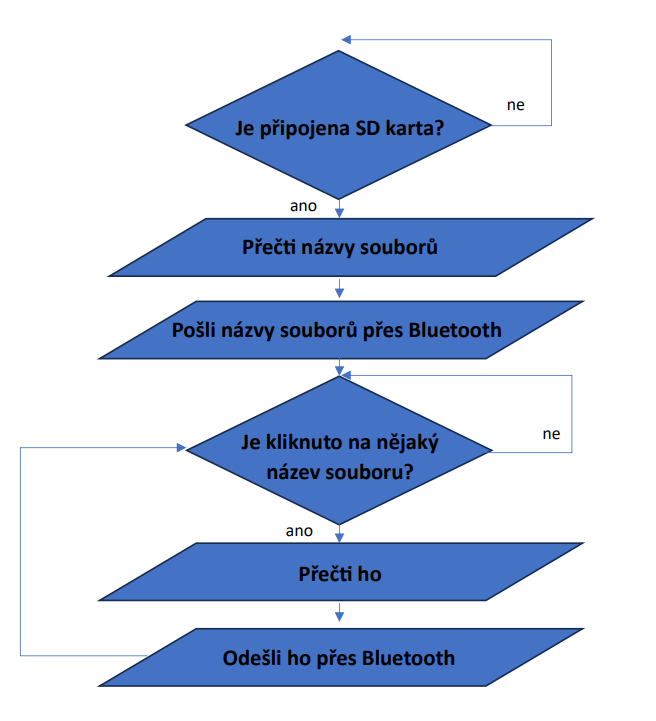
\includegraphics[width=0.5\textwidth]{images/vyvojovy_diagram.png}
        \caption{Vývojový diagram znázorňující chod programu na Arduinu}
    \end{figure}

    \begin{figure}[H]
        \centering
        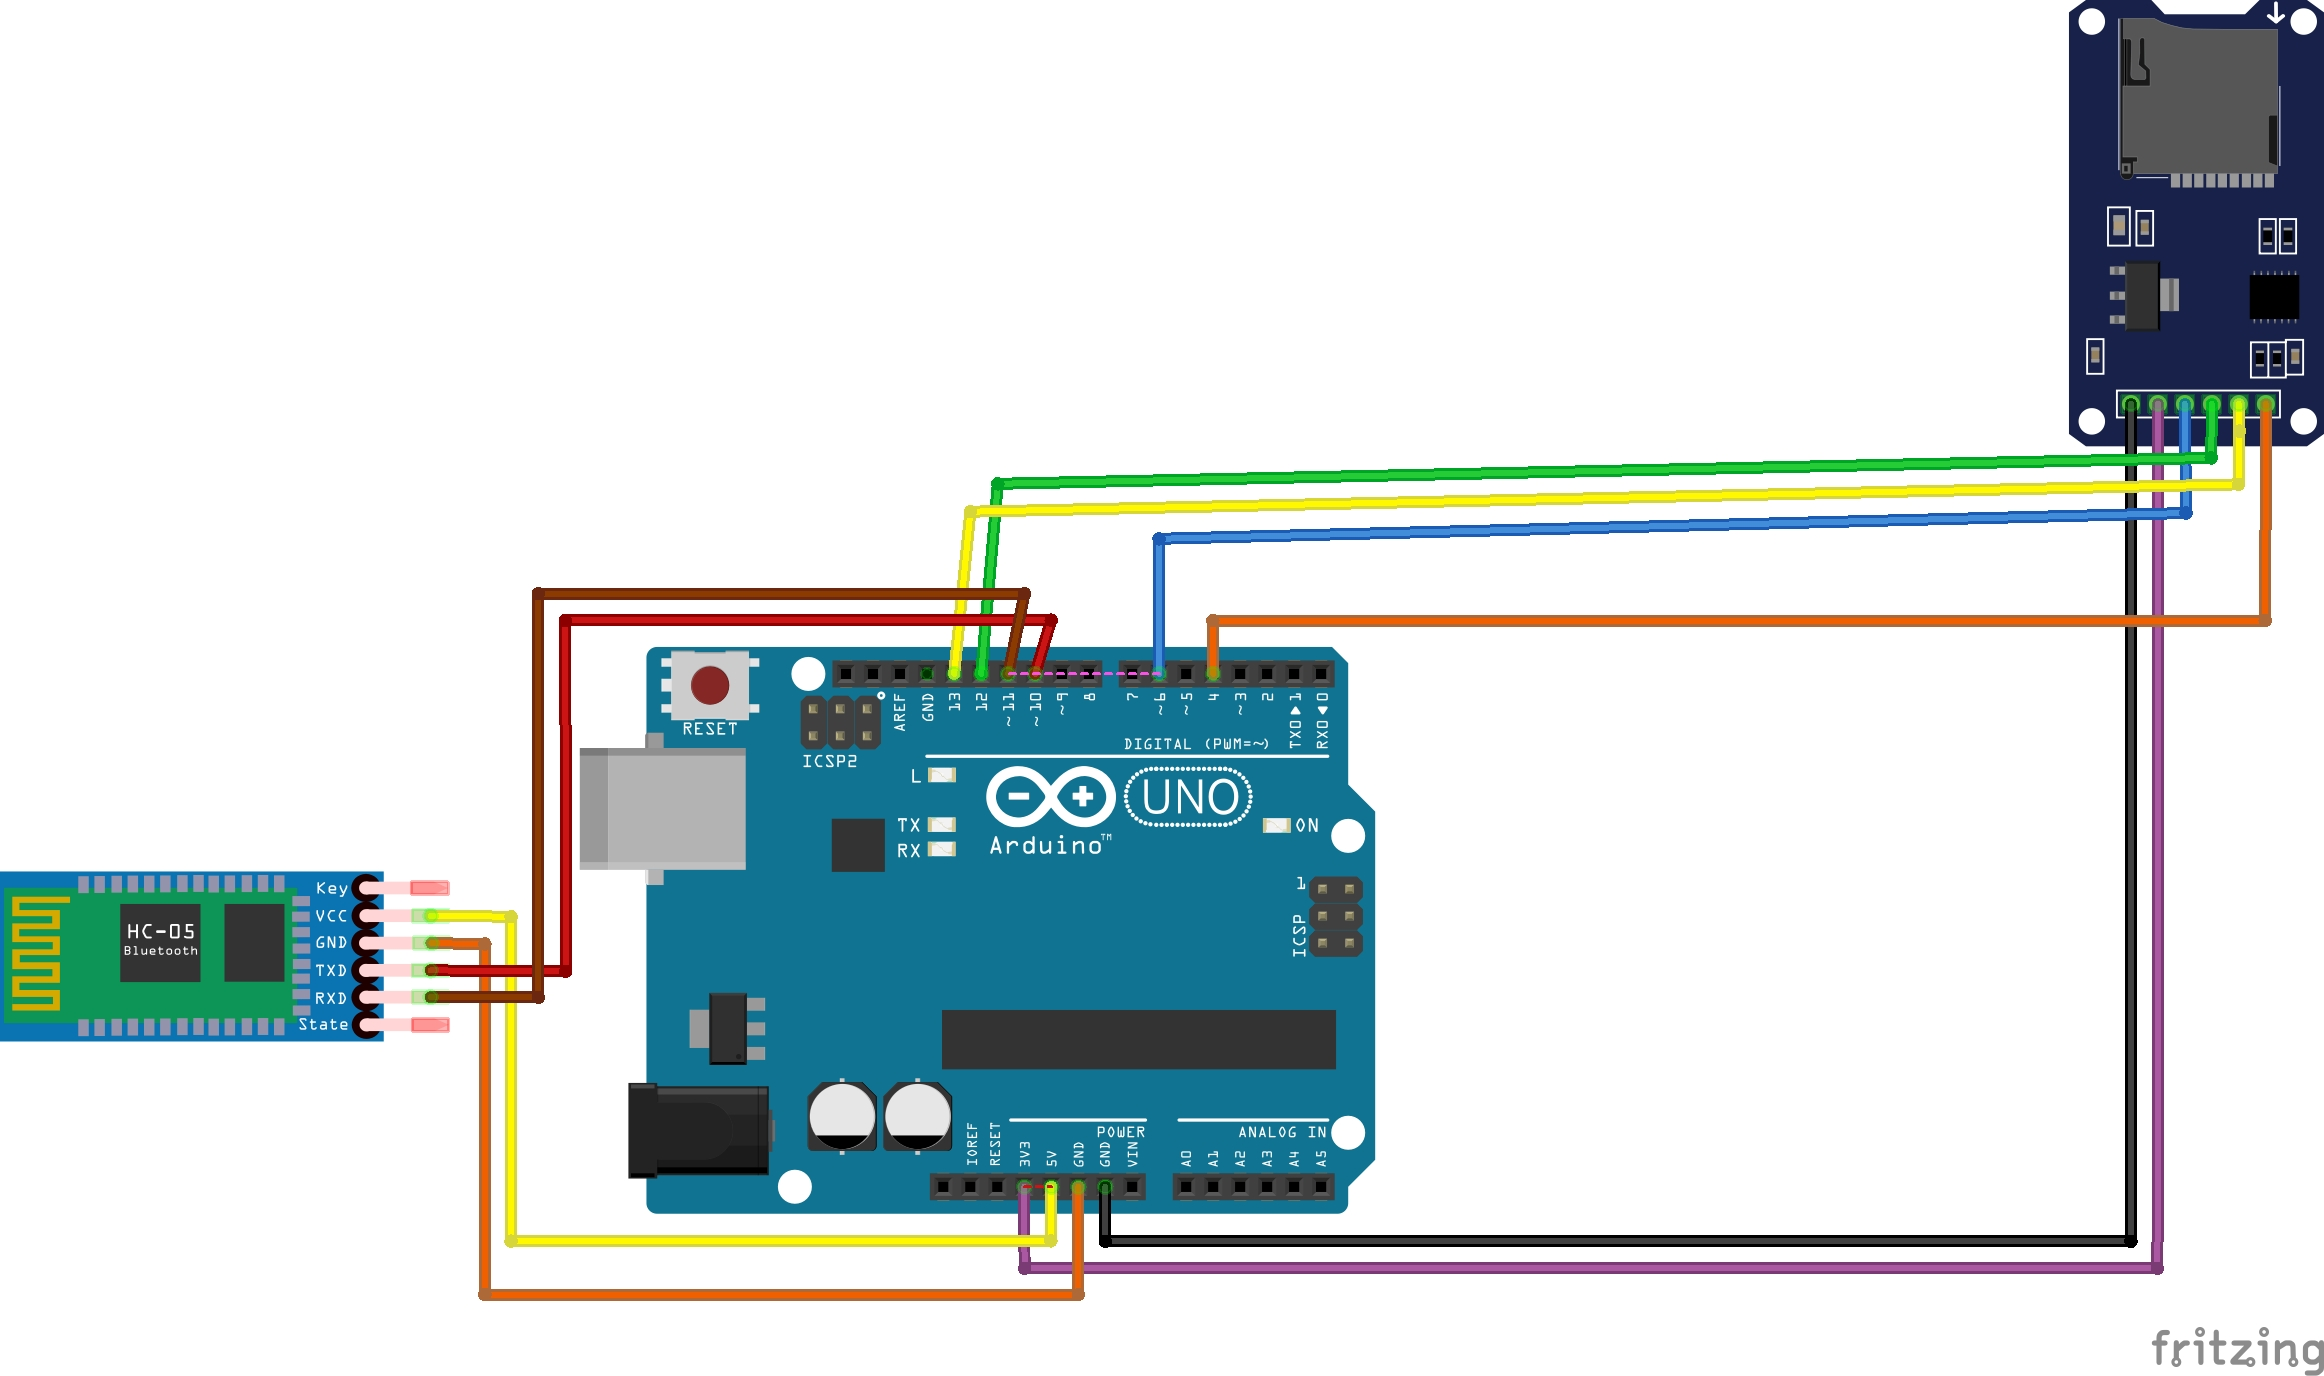
\includegraphics[width=0.5\textwidth]{images/schema_zapojeni.jpg}
        \caption{Schéma zapojení součástek k Arduinu}
    \end{figure}
    
\end{itemize}
